\documentclass[pdf,hyperref={urlbordercolor={0 1 1}},xcolor=pdftex,dvipsnames]{beamer}

\mode<presentation>
{
  \usetheme{Golm}
  \setbeamercovered{transparent}
}

\usepackage[english]{babel}
\usepackage[latin1]{inputenc}
\usepackage{times}
\usepackage[T1]{fontenc}
\usepackage{pifont}
\usepackage{amsmath,amssymb,curves,epic,cancel}
\usepackage{tikz}
\usepackage{multirow}
\usepackage{scalefnt}
\usetikzlibrary{decorations.pathreplacing}
\usetikzlibrary{automata,positioning}

%\setbeamercolor{math text}{fg=blue!50!black}

\beamertemplatenavigationsymbolsempty

\title[Ramsey Theory: Computational Approaches]
{Computational Approaches\\ to Ramsey Problems}

\author[Alex Weinstock-Collins \& Ethan Mark]
  {{Alex Weinstock-Collins\\\vspace{.1cm} \& Ethan Mark}\\
}

\date{
  REU Week 2 Report\\ \vspace{.25cm}
  June 14, 2013
}

\AtBeginSection[]
{
  \begin{frame}<beamer>
    \frametitle{Outline}
    \addtocounter{framenumber}{-1}
    \tableofcontents[currentsection]
  \end{frame}
}

\begin{document}

%Title Page
\begin{frame}
  \titlepage
\end{frame}

%Outline
\begin{frame}
  \frametitle{Outline}
  \tableofcontents
\end{frame}

\section{Graph Generation}

\begin{frame}
  \frametitle{Ramsey Theory Review}
  \textit{Recall:}. \\\vspace{.25cm}
 \textbf{Ramsey Number} $R(n_1,....,n_c)=r$ is the minimum order of a complete graph in $c$ colors that must contain a complete subgraph of order  $n_i$ whose edges are all color $i$.  \\\vspace{.25cm}
\textbf{Bipartite Ramsey Number}: $b(n_1,...,n_k)$ is the smallest number $b$ such that any coloring of the edges of $K_{b,b}$, with $k$ colors guarantees a monochromatic copy of $K_{n_i,n_i}$, in the $i$-th color, for some $i$, $1\le i \le k$.\\\vspace{.25cm} 
\textbf{Zarankiewicz Numbers}: $z(m,n;s,t)$ is the maximum number of edges in a subgraph of $K_{m,n}$ that does not contain $K_{s,t}$ as a subgraph. \\\vspace{.25cm}
\end{frame}
\begin{frame}
  \frametitle{Nauty}
 \textbf{nauty} created in 1984 is a program for creating and computing graphs. \\\vspace{.25cm}
Examples: \\\vspace{.25cm}
Generating complete graphs or bipartite graphs. \\\vspace{.25cm}
Counting graphs with certain properties. \\\vspace{.25cm}


  % -how we can use nauty to improve lower bounds on small Ramsey-type numbers
\end{frame}

\begin{frame}
  \frametitle{Limits of nauty}
  How long nauty took to generate $C_4$-free bipartite graphs.
  \begin{center}\begin{tabular}{| c | c | c | c |}\hline
    \multirow{2}{*}{Vertices} & \multirow{2}{*}{Edges} & Graphs & 
      \multirow{2}{*}{Time Taken} \\
    & & Generated & \\\hline\hline
    16 & 24 & 4\footnote{Includes three subgraphs of $K_{8,8}$ and one subgraph of
      $K_{7,9}$, since $z(8,8)=z(7,9)=24$ and nauty does not allow specification of
      vertex allocation.} & 1.11 seconds \\\hline
    18 & 29 & 1 & 15.90 seconds \\\hline
    20 & 34 & 1 & $\approx5.5$ minutes \\\hline
    22 & 39 & 2\footnote{One subgraph of $K_{11,11}$, one of $K_{10,12}$, 
      $z(11,11)=z(10,12)=39$.} & $\approx3$ hours \\\hline
  \end{tabular}\end{center}
  This technique will only be useful for diagonal Zarankiewicz numbers.
\end{frame}

\section{Examples}

\begin{frame}
  \frametitle{The unique witness for $z(9,9)=29$}
  \begin{center}
    \begin{minipage}[c]{.47\textwidth}
      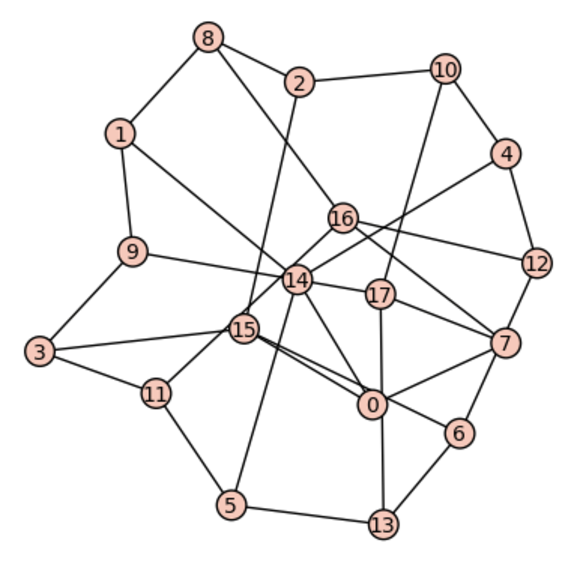
\includegraphics[scale=.5]{figs/b18z29.pdf}
    \end{minipage}
    \begin{minipage}[c]{.47\textwidth}
      \begin{center}
        {\scalefont{.35}
          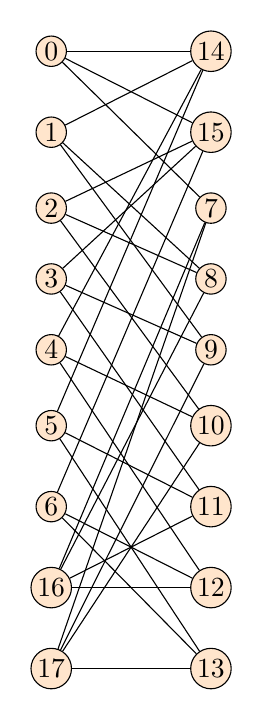
\begin{tikzpicture}
            \matrix[nodes={draw, circle, fill=orange!20}, 
    row sep=.5cm, column sep=1.5cm, inner sep=1pt, minimum size=.25cm]{
  \node (v0) {0}; & \node (v14) {14}; \\
  \node (v1) {1}; & \node (v15) {15}; \\
  \node (v2) {2}; & \node (v7) {7}; \\
  \node (v3) {3}; & \node (v8) {8}; \\
  \node (v4) {4}; & \node (v9) {9}; \\
  \node (v5) {5}; & \node (v10) {10}; \\
  \node (v6) {6}; & \node (v11) {11}; \\
  \node (v16) {16}; & \node (v12) {12}; \\
  \node (v17) {17}; & \node (v13) {13}; \\
};
\foreach \u/\v in {v0/v7,v0/v14,v0/v15,v1/v8,v1/v9,v1/v14} \draw (\u) -- (\v);
\foreach \u/\v in {v2/v8,v2/v10,v2/v15,v3/v9,v3/v11,v3/v15} \draw (\u) -- (\v);
\foreach \u/\v in {v4/v10,v4/v12,v4/v14,v5/v11,v5/v13,v5/v14} \draw (\u) -- (\v);
\foreach \u/\v in {v6/v12,v6/v13,v6/v15,v17/v7,v17/v9,v17/v10} \draw (\u) -- (\v);
\foreach \u/\v in {v17/v13,v16/v7,v16/v8,v16/v11,v16/v12} \draw (\u) -- (\v);

          \end{tikzpicture}
        }
      \end{center}
    \end{minipage}
  \end{center}
\end{frame}

\begin{frame}
  \frametitle{The unique witness for $z(10,10)=34$}
  \begin{center}
    \begin{minipage}[c]{.47\textwidth}
      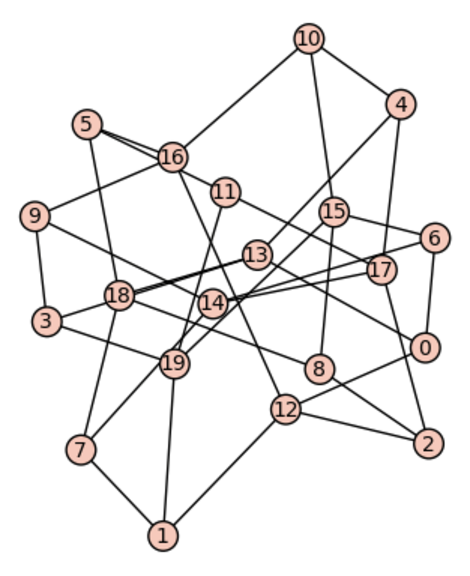
\includegraphics[scale=.5]{figs/b20z34.pdf}
    \end{minipage}
    \begin{minipage}[c]{.47\textwidth}
      \begin{center}
        {\scalefont{.35}
          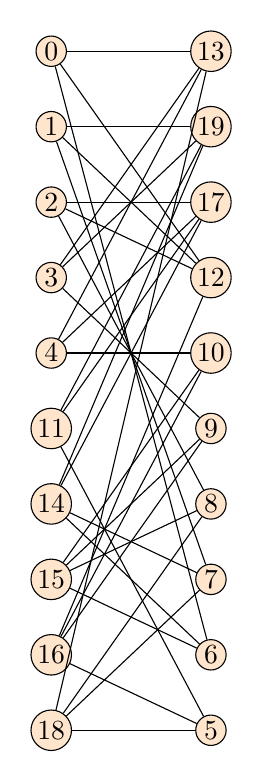
\begin{tikzpicture}[scale=.5]
            \matrix[nodes={draw, circle, fill=orange!20}, 
    row sep=.43cm, column sep=1.5cm, inner sep=1pt, minimum size=.25cm]{
  \node (v0) {0}; & \node (v13) {13}; \\
  \node (v1) {1}; & \node (v19) {19}; \\
  \node (v2) {2}; & \node (v17) {17}; \\
  \node (v3) {3}; & \node (v12) {12}; \\
  \node (v4) {4}; & \node (v10) {10}; \\
  \node (v11) {11}; & \node (v9) {9}; \\
  \node (v14) {14}; & \node (v8) {8}; \\
  \node (v15) {15}; & \node (v7) {7}; \\
  \node (v16) {16}; & \node (v6) {6}; \\
  \node (v18) {18}; & \node (v5) {5}; \\
};
\foreach \u/\v in {v0/v6,v0/v12,v0/v13,v1/v7,v1/v12,v1/v19} \draw (\u) -- (\v);
\foreach \u/\v in {v2/v8,v2/v12,v2/v17,v3/v9,v3/v13,v3/v19} \draw (\u) -- (\v);
\foreach \u/\v in {v4/v10,v4/v13,v4/v17,v11/v5,v11/v19,v11/v17} \draw (\u) -- (\v);
\foreach \u/\v in {v14/v6,v14/v7,v14/v19,v14/v17,v15/v6,v15/v8} \draw (\u) -- (\v);
\foreach \u/\v in {v15/v10,v15/v9,v16/v5,v16/v9,v16/v10,v16/v12} \draw (\u) -- (\v);
\foreach \u/\v in {v18/v5,v18/v7,v18/v8,v18/v13} \draw (\u) -- (\v);

          \end{tikzpicture}
        }
      \end{center}
    \end{minipage}
  \end{center}
\end{frame}

\section{Other Techniques}

\begin{frame}
  \frametitle{Zarankiewicz numbers to check}
  \begin{center}
    \begin{tikzpicture}
      \node[anchor=south west, inner sep=0pt, outer sep=0pt]
        (image) at (0,0) {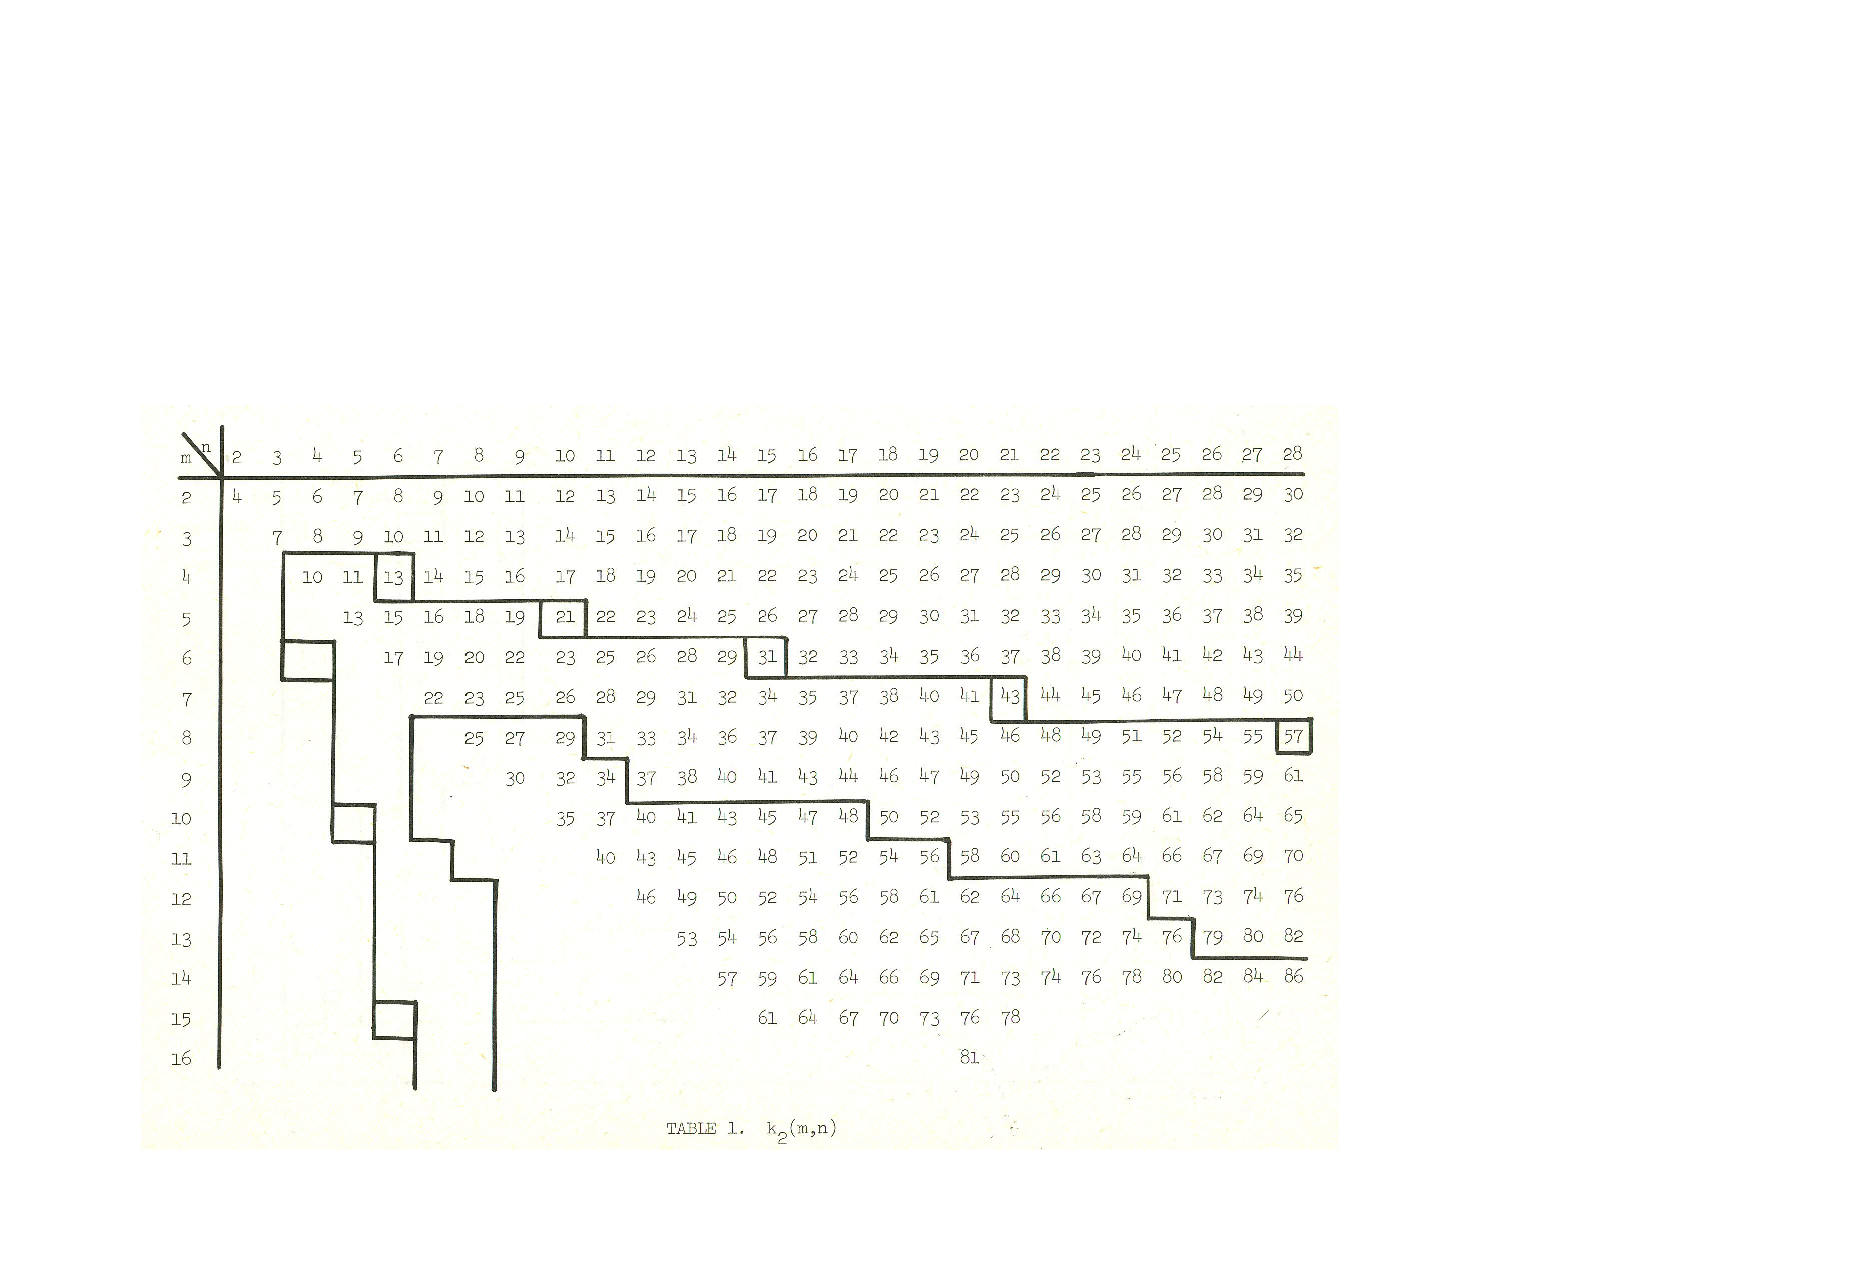
\includegraphics[scale=.5]{figs/ZaranTables.pdf}};
      \draw[color=red] (5.3,1.12) circle (.15cm);
      \draw[color=blue] (3.65,2.7) -- (5.1,4.1);
    \end{tikzpicture}
  \end{center}
\end{frame}

\begin{frame}[noframenumbering]
  \frametitle{Zarankiewicz numbers to check}
  \begin{center}
    \begin{minipage}[b]{.47\textwidth}
      \begin{tikzpicture}
        \node[anchor=south west, inner sep=0pt, outer sep=0pt]
          (image) at (0,0) {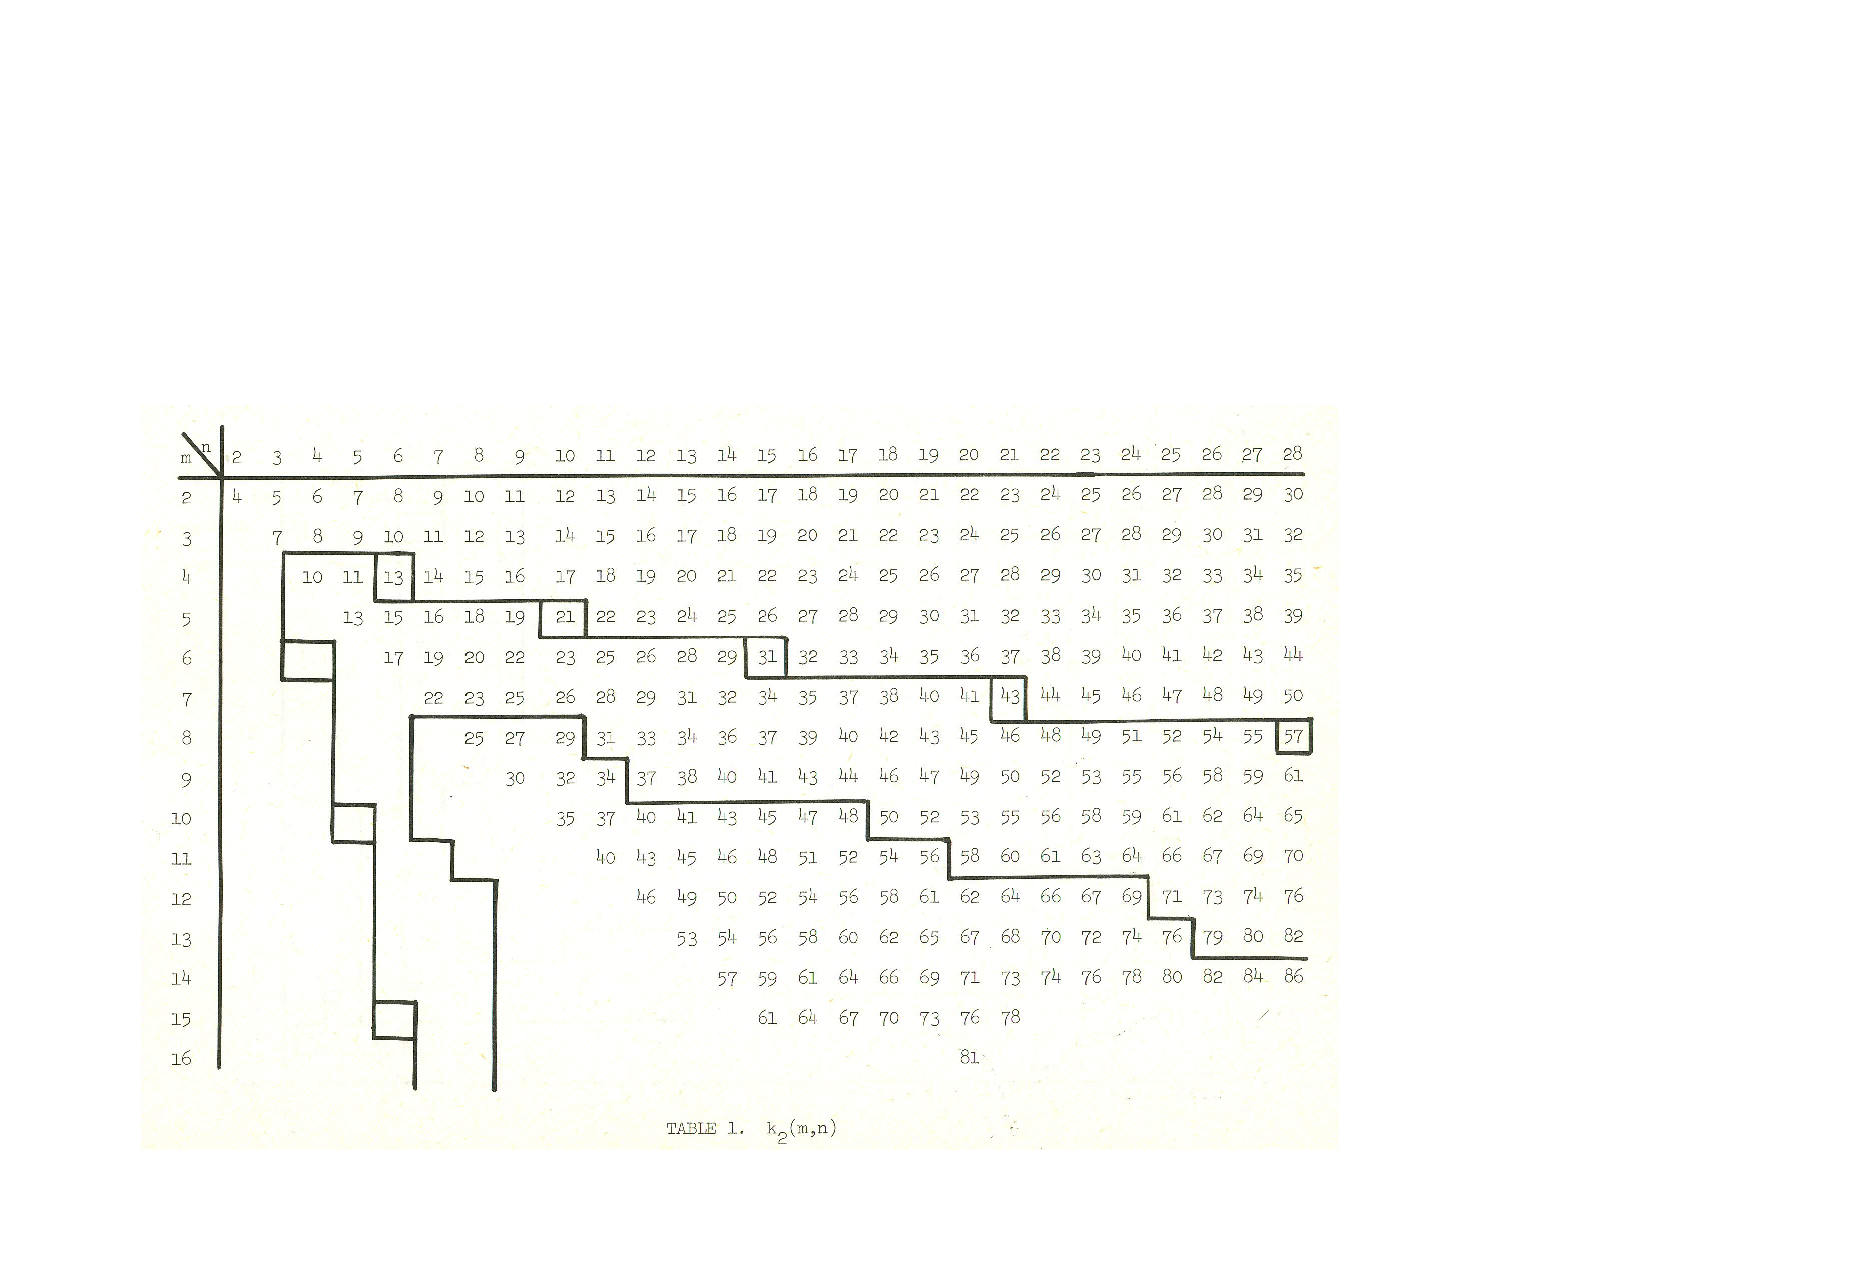
\includegraphics[scale=.25]{figs/ZaranTables.pdf}};
        \draw[color=red] (2.65,.56) circle (.075cm);
        \draw[color=blue] (1.825,1.35) -- (2.55,2.05);
      \end{tikzpicture}
    \end{minipage}
    \begin{minipage}[b]{.47\textwidth}
      \begin{itemize}
        \item From Guy, 1969
        \item Values are $z(n,m)+1$ due to alternate definition
        \item Values above top line determined by easily verifiable theorem
      \end{itemize}
    \end{minipage}
    \begin{itemize}
      \item Values between lines determined by other theorem (proof missing)
      \item Other values determined by individual argument
      \item Circled value does not match newer paper (Dybizba\'nski, Dzido, 
        Radziszowski, 2013)
      \item Values beyond blue line are not feasibly checkable by nauty
    \end{itemize}
  \end{center}
\end{frame}

\begin{frame}[noframenumbering]
  \frametitle{Zarankiewicz numbers to check}
  \begin{minipage}[b]{.52\textwidth}
    \begin{center}
      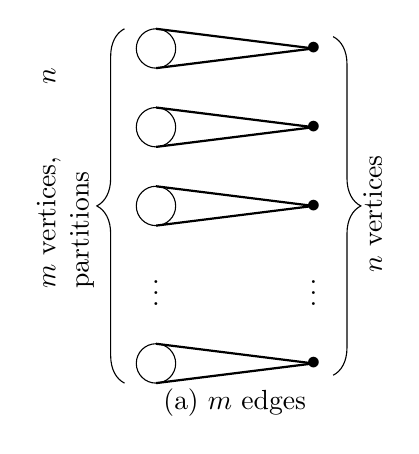
\begin{tikzpicture}[scale=.5]
  \draw (0,0) circle(.5cm);
  \node at (0,2) (ds) {$\vdots$};
  \draw (0,4) circle(.5cm);
  \draw (0,6) circle(.5cm);
  \draw (0,8) circle(.5cm);
  \node at (4,8) (v0) {$\bullet$};
  \node at (4,6) (v1) {$\bullet$};
  \node at (4,4) (v2) {$\bullet$};
  \node at (4,2) (dv) {$\vdots$};
  \node at (4,0) (vn) {$\bullet$};
  \draw [decorate, decoration={brace, amplitude=10pt}] (-.8,-.5) -- (-.8,8.5) 
    node [midway, %anchor=east, 
      xshift=-.75cm, yshift=.45cm, 
      text width=3cm, rotate=90] 
    {$m$ vertices,\hspace{.8cm} $n$ partitions};
  \draw [decorate, decoration={brace, amplitude=10pt, mirror}] (4.5,-.3) -- (4.5,8.3) 
    node [midway, %anchor=west, 
      xshift=.5cm, yshift=-.1cm, 
      rotate=90] {$n$ vertices};
  \draw [thick] (4,8) -- (0,8.5);
  \draw [thick] (4,8) -- (0,7.5);
  \draw [thick] (4,6) -- (0,6.5);
  \draw [thick] (4,6) -- (0,5.5);
  \draw [thick] (4,4) -- (0,4.5);
  \draw [thick] (4,4) -- (0,3.5);
  \draw [thick] (4,0) -- (0,.5);
  \draw [thick] (4,0) -- (0,-.5);
  \node at (2,-1) (label) {(a) $m$ edges};
\end{tikzpicture}

    \end{center}
  \end{minipage}
  \begin{minipage}[b]{.44\textwidth}
    \begin{center}
      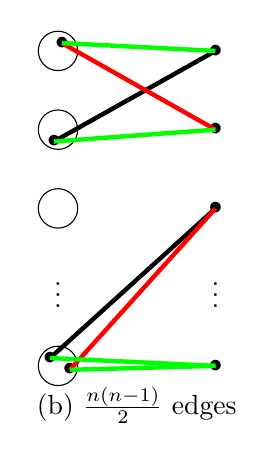
\begin{tikzpicture}[scale=.5]
  \draw (0,0) circle(.5cm);
  \node at (0,2) (ds) {$\vdots$};
  \draw (0,4) circle(.5cm);
  \draw (0,6) circle(.5cm);
  \draw (0,8) circle(.5cm);
  \node at (4,8) (v0) {$\bullet$};
  \node at (4,6) (v1) {$\bullet$};
  \node at (4,4) (v2) {$\bullet$};
  \node at (4,2) (dv) {$\vdots$};
  \node at (4,0) (vn) {$\bullet$};
  \node at (2,-1) (label) {(b) $\frac{n(n-1)}2$ edges};
  \node at (.1,8.2) (u0) {$\bullet$};
  \node at (-.1,5.7) (u1) {$\bullet$};
  \node at (-.2,.2) (u2) {$\bullet$};
  \node at (.3,-.1) (u3) {$\bullet$};
  \draw [ultra thick] (4,8) -- (-.1,5.7);
  \draw [ultra thick, red] (4,6) -- (.1,8.2);
  \draw [ultra thick] (4,4) -- (-.2,.2);
  \draw [ultra thick, red] (4,4) -- (.3,-.1);
  \draw [ultra thick, green] (4,8) -- (.1,8.2);
  \draw [ultra thick, green] (4,6) -- (-.1,5.7);
  \draw [ultra thick, green] (4,0) -- (-.2,.2);
  \draw [ultra thick, green] (4,0) -- (.3,-.1);
\end{tikzpicture}

    \end{center}
  \end{minipage}
  \textit{Theorem} (Guy, 1968): $z(n,m)=m+\binom{n}{2}$ for $m>\binom{n}{2}$.
\end{frame}

\begin{frame}
  \frametitle{Alternative methods}
  Algorithm for checking Zarankiewicz numbers:
  \begin{itemize}
    \item Begin with $n,m~(n\le m)$ and $z$, a guess at $z(n,m)$ to check
    \item Generate all possible degree sequences of the $n$ vertices on the
      left which add up to $z$.
    \item Eliminate all theoretically impossible sequences
    \begin{itemize}
      \item Denote the degree sequence $S=(s_0,s_1,\ldots,s_{n-1})$
      \item Let $\Delta_k=\sum_{i=0}^{k-1}s_i$
      \item If $\Delta_k>m+\binom{k}{2}$, then the degree sequence can be 
        eliminated (generalization of prior theorem)
    \end{itemize}
    \item Check all remaining (theoretically possible) degree sequence
  \end{itemize}
  Note: Still working on last step
\end{frame}

\section{Projective Planes}

\begin{frame}
  \frametitle{Projective Planes}
  What are they?\\Why are they useful?
\end{frame}

\begin{frame}
  \frametitle{Readings}
  % TODO
\end{frame}

\begin{frame}
  \frametitle{Questions}
  \begin{center}
    {\Large Questions?}
  \end{center}
\end{frame}

\end{document}



